\section{Experimental Results}
\label{sec:results}

\paragraph{The choice of scene understanding levels. }
\label{results:levels}
We evaluate the algorithms at three granularity levels for each object category: coarse-, middle- and fine-grained, roughly corresponding to evaluation in~\cite{mo2019partnet}. 
Because of arbitrary nature of part labels in the PartNet dataset, metric scale doesn't always correspond to levels of object taxonomy. We choose to train on first 3 levels of object taxonomy to minimize discrepancy in geometry for levels >= 4.
Here are main guiding principles for levels of detail selection in a general case:
\begin{itemize}
    \item The higher the number of classes the lower segmentation performance of the model
    \item The higher the number of voxels for a given label class the higher prediction accuracy of that class
    \item The lower the level of detail the simpler geometry of parts on that level 
\end{itemize}

\begin{wraptable}{r}{5.5cm}
\caption{Model configurations that we consider, with $\alpha_i$ in~\eqref{eq:semseg_loss}.}
\begin{tabular}{lrrr}\\\toprule  
Configuration   & $\alpha_1$ & $\alpha_2$ & $\alpha_3$ \\
\midrule
Base coarse     & 1 & 0 & 0 \\
Base middle     & 0 & 1 & 0 \\
Base fine       & 0 & 0 & 1 \\
MTT-12          & .5 & .5 &  0 \\
MTT-123-coarse  & .5 & .3 & .2 \\
MTT-123-fine    & .2 & .3 & .5 \\
\bottomrule
\end{tabular}
\label{table:configurations}
\end{wraptable} 


Trying to find the optimal trade-off between principle described above we concluded that all of the relevant information will be preserved if we work with hierarchy levels equal or lower than 3, and minimum number of voxels for a given class equal to 1800.

% TODO describe oracle and greedy mode, as equations, 


\paragraph{Quality measures. }
\label{results:metrics}
We evaluate semantic labeling and hierarchical segmentation models by inferring the semantic labels for entire input scenes and computing quality measures at each scene understanding level $d_k$ separately. 
More specifically, for each class $c$ present in the set of classes $\mathbb{C}_k$ at granularity $d_k$, we compute the standard Intersection over Union score $\text{IoU}_c$ and the balanced accuracy score $\text{Acc}_c$.
We report these per-class numbers along with mean IoU and mean balanced accuracy averaged over $\mathbb{C}_k$: $\text{mIoU}_k = \sfrac{1}{n_k}\sum_{c \in \mathbb{C}_k} \text{IoU}_c$, $\text{mAcc}_k = \sfrac{1}{n_k}\sum_{c \in \mathbb{C}_k} \text{Acc}_c$.

We additionally evaluate hierarchical semantic segmentation by averaging mIoU over all hierarchy levels $k \in \{1, \ldots, K\}$.

Instance segmentation is assessed as object detection and thus evaluate this task using average precision (AP) with IoU threshold at 0.5. To generate object hypotheses, each instance is checked against a threshold of confidence equal to 0.25, to filter out noisy voxels.

% Hierarchical models are evaluated somewhat differently. Specifically, we consider how categorical predictions of parts are combined to provide prediction of classes on some level of detail. 

% Ensemble models are evaluated by combining predictions either from different output "heads" of the model or from outputs of several separately trained models. 

% For Bottom-up approach - each "head" is evaluated separately, test set predictions are collected in a confusion matrix $C=(c_{ij}), i=1..N_C, j=1..N_C$, where $N_C$ is a number of classes of a certain "head". $TP_i = c_{ii}$ - is a number of true positives, $FP_i = \sum_{j=1..N_C} c_{ji} - TP_i$  is the number of false positives, and $FN_i = \sum_{j=1..N_C} c_{ij} - TP_i$ are false positive samples.
% We use the standard Intersection over Union (IoU) score defined as $\text{IoU}_c = \sfrac{TP_c}{(TP_c + FP_c + FN_c)}$ for class $c$ as well as a mean IoU.
% Balanced accuracy score~\cite{brodersen2010balanced} defined as average of per-class recall values $R_i$.
% \[
% R_i = \frac{TP_i}{TP_i + FN_i}
% \]
% is also computed. 

\paragraph{Part-level semantic labeling results. }
\label{results:semseg}
We first study part-level semantic labeling performance at different granularity levels $d_1, d_2, d_3$ in Table~\ref{tab:semseg}. 

We found that in some cases we can achieve a better performance than a baseline by evaluating model on lower level of details and projecting labels up through hierarchy. If $p_i^{d_j}$ - probability of a given voxel to have a class label $C_i^{d_j}$ where $i=1...n_j$ and $d_j, j=1, 2, 3$ - signifies the level of granularity, $Parent(i, d_j)$ - function that returns parent class index given child class index $i$ on the level $d_j$, because part hierarchy is a tree without isolated nodes, function always returns a single class index. Consequently the prediction labels projected up will be:
\begin{equation}
C_t^{d_{j-1}} = Parent\left(\argmax_{i=1...n_j}(p_i^{d_j}), d_j\right) .
\end{equation}

To improve prediction on a specific level of granularity we can train models in multitask setting which have shown their peak performance on multiple level of granularity. For example the MTT-12 and MTT-123-coarse have outperformed the base-coarse model on $d_1$, and the MTT-123-fine have outperformed base-fine model on $d_3$.
From that we can conclude that changing distribution of weights to different heads in multi-task setting trades performance across levels of details. Maximum value of weight in table~\ref{table:configurations} for the loss function term in~\eqref{eq:semseg_loss} roughly predicts level of detail with best performance.

\begin{figure}[!t]
\label{fig:experiments_visual}
\centering
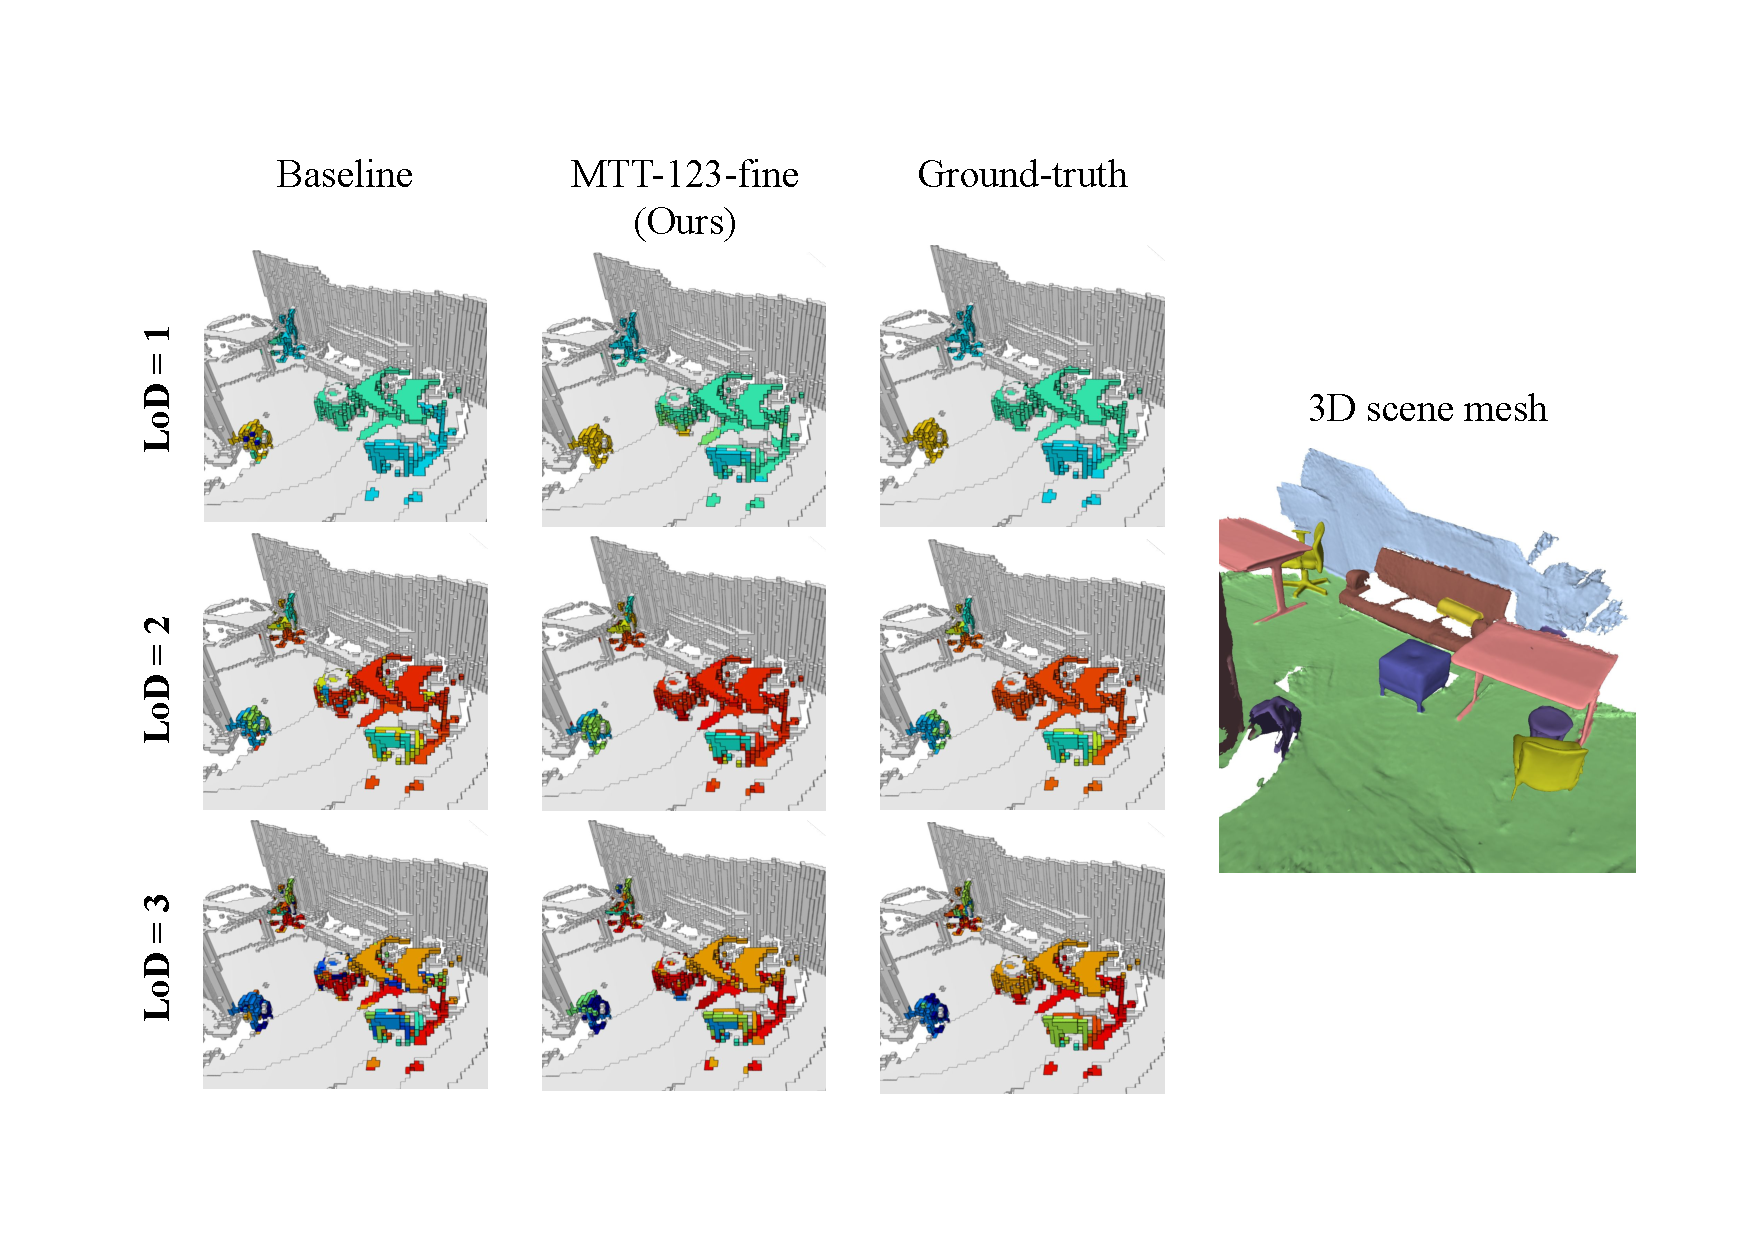
\includegraphics[width=0.99\textwidth]{Figures/scan2part/experiments_visual.pdf}
\caption{Qualitative hierarchical semantic segmentation results using the baseline models trained in each respective part-category level and our proposed method. Note the improved segmentation performance, particularly at finer levels in the parts taxonomy (lower row).}
\label{fig:hierarchical_seg_visual}
\end{figure}

\begin{table}[!h]

\caption{Part-level semantic segmentation performance in terms of mean IoU and mean balanced accuracy for different semantic granularities.}
\centering
\begin{tabular}{l rrr rrrr}
\toprule
 & \multicolumn{3}{c}{mAcc,\,\% $\uparrow$} && \multicolumn{3}{c}{mIoU,\,\% $\uparrow$} \\
\cmidrule{2-4}
\cmidrule{6-8}
Configuration   & $d_1$ & $d_2$ & $d_3$ && $d_1$ & $d_2$ & $d_3$ \\
\midrule
Base coarse     &  62.6 & ---   & ---   &&  22.5 & ---   & ---   \\
Base middle     &  \textbf{64.1} &  \textbf{57.9} & ---   &&  23.0 &  13.1 & ---   \\
Base fine       &  54.2 &  47.1 &  31.0 &&   9.5 &  \textbf{17.7} &   5.8 \\
% Base coarse (nw) & 71.74 & --- & --- & 27.15 & --- & --- \\
% Base coarse (bg) & 88.78 & --- & --- &  1.8  & --- & --- \\
\midrule
MTT-12          &  63.4 &  53.5 & ---   &&  \textbf{28.7} &  15.9 & ---   \\
MTT-123-coarse  &  63.5 &  56.2 &  32.5 &&  23.3 &  12.0 &   6.3 \\
MTT-123-fine    &  60.7 &  52.6 &  \textbf{34.7} &&  21.9 &  12.1 &   \textbf{6.7} \\
\midrule
Num. classes    &    13 &    36 &    79 &&    13 &    36 &    79 \\
\bottomrule
\end{tabular}
\label{tab:semseg}

\end{table}

\paragraph{Hierarchical semantic segmentation results. }
\label{results:hierarhical}
We present performance of hierarchical semantic segmentation in Table~\ref{tab:hierarchical_seg} and display these visually in Figure~\ref{fig:hierarchical_seg_visual}. Note that despite the baselines are focusing solely on their respective level of semantic detail, our methods is able to leverage a multi-task objective in~\eqref{eq:semseg_loss} to perform more efficient segmentation.

Hierarchical semantic segmentation is performed in a similar fashion to segmentation in MTT setting, but instead of classification of each voxel on each level of detail, heads in hierarchical model are more numerous (51 head) and perform classification of voxels to a specific sub-part class of parent class, e.g. classifying presumed chair shape to chair back, legs and seat. In this setting model is evaluated in two modes:
\begin{itemize}
    \item Oracle - in this mode mask of the parent class is taken from the ground truth data, thus each head is evaluated on it's ability to classify specific sub-parts of a certain object on specific level of detail. 
    \item Greedy - when parent object mask is predicted by heads higher in the hierarchy, predictions of the root node in hierarchy is performed first, masks for the objects are computed and heads lower on the tree evaluated only on respective mask. In this way model is evaluated as a whole top-down, which can lead to compounding of errors.
\end{itemize}
The results in Table~\ref{tab:hierarchical_seg} tell us that hierarchical model can segment specific sub-parts of many objects reasonably well. The problem arises when we try to integrate the predictions one after another in a sequential decision process, causing errors to compound and become incorrect the deeper in the tree they go.

\begin{table}[!h]

\caption{Hierarchical semantic segmentation results in terms of mean IoU and mean balanced accuracy for different semantic granularities. We include mIoU averaged over all hierarchy levels as an integral measure.}
\centering
\begin{tabular}{l rrrr r rrrr}
\toprule
  & \multicolumn{4}{c}{mAcc,\,\% $\uparrow$} 
 && \multicolumn{4}{c}{mIoU,\,\% $\uparrow$} \\
\cmidrule{2-5}
\cmidrule{7-10}
Configuration           & $d_1$ & $d_2$ & $d_3$ &  avg. && $d_1$ & $d_2$ & $d_3$ & avg. \\
\midrule
**Oracle (top-down)        &  58.5 &  82.0 &  70.9 &  70.5 &&   15.8 &  43.3 &  36.2& 31.8 \\
\midrule
Base fine (bottom-up)    &  54.2 &  47.1 &  31.0 &  44.1 &&   9.5 &  \textbf{17.7} &   5.8 & 11.0 \\
Greedy (top-down)        &  30.9 &  16.4 &   9.2 &  18.8 &&  19.0 &   9.2 &   4.8 & 11.0 \\
MTT-123-coarse           &  \textbf{63.5} &  56.2 &  32.5 &  50.7 &&  \textbf{23.3} &  12.0 &   6.3 & \textbf{13.9} \\
MTT-123-fine             &  60.7 &  52.6 &  34.7 &  49.4 &&  21.9 &  12.1 &  \textbf{6.7} & 13.6 \\
MTT-123-coarse (ensemble)&  \textbf{63.5} &	\textbf{56.8} &	33.8 & \textbf{51.4} &&   \textbf{23.3} &  11.6 &   6.1 & 13.7 \\
MTT-123-fine (ensemble)  & 60.7	 & 53.1 &	\textbf{35.6} & 49.8 &&   21.9 &  11.7 &   6.6 & 13.4 \\
\midrule
Num. classes            &    13 &    36 &    79 &       &&    13 &    36 &    79 &      \\
\bottomrule
\end{tabular}
\label{tab:hierarchical_seg}
\end{table}


\paragraph{Part instance segmentation results. }
\label{results:instance}
We present instance segmentation results in Table~\ref{table:instance}.

As expected performance of instance segmentation drops with reduction of level of detail, caused mainly by the loss of the unique properties of the instance masks, and lowering of the mean number of the voxels per instance mask.

Because we have $d_1$ level object instance mask and semantic part masks, to create $d_2, d_3$ instance masks we have a pre-processing step that selects unique semantic masks for each object instance mask separately.

\begin{table}[!h]

\caption{Instance segmentation performance in terms of mean IoU for varying levels of detail (LoD).}
\centering
\begin{tabular}{lrrr}
\toprule
Configuration       & mIoU,\,\% & AP@50,\,\%    & AR@50,\,\% \\ 
\midrule
Base coarse         & \textbf{78.6}     & \textbf{83.9} & \textbf{35.9} \\
% LoD=1, bg-push & \textbf{80.56\%} & 74.50\% & \textbf{37.11\%} \\
Base middle         & 70.5     & 54.2         & 16.6 \\
Base fine           & 64.7     & 41.4         & 15.4 \\
\bottomrule
\end{tabular}%
\label{table:instance}

\end{table}

